\subsection{HiC Plotter}\label{HiC:hicplotter}% __13a-hicplotter
%~~~~~~~~~~~~~~~~~~~%
\subsubsection{Input} % inputs
Data from the pipeline steps %\texttt{matrix-estimated}) (Section~\ref{HiC:matrix-estimated}), % this one removed
\texttt{matrix-filtered} (Section~\ref{HiC:matrix-filtered}), \texttt{matrix-hicnorm} (Section~\ref{HiC:matrix-hicnorm}), \texttt{matrix-prep} (Section~\ref{HiC:matrix-prep}), and \texttt{matrix-ic} (Section~\ref{HiC:matrix-ic}) are used as input.
%~~~~~~~~~~~~~~~~~~~%
\subsubsection{Analysis} % analysis
Default parameters:
\begin{lstlisting}
params.standard.tcsh$
#!/bin/tcsh

source ./inputs/params/params.tcsh

# HiCplotter path
set hicplotter_path = ./code/HiCPlotter2.py

# create bedgraphs for boundary scores
set bscores_branch = ../boundary-scores/results/boundary-scores.by_sample.standard/`echo $branch | sed 's/.*results\///'`
set cell_type = `echo $objects[1] | cut -d'-' -f1`
set f = $bscores_branch/$objects[1]/all_scores.k=001.tsv
set methods = (intra-max DI ratio)
set bedgraphs = ()
set bedgraph_labels = ($methods)
foreach m ($methods)
  set k = `head -1 $f | tr '\t' '\n' | grep -n "^$m"'$' | cut -d':' -f1`
  cat $f | sed '1d' | cut -f1,$k | sed 's/:/\t/' | sed 's/-/\t/' >! $outdir/bscores.$m.bedGraph
  set bedgraphs = ($bedgraphs $outdir/bscores.$m.bedGraph)
end

# add CTCF ChIP-seq
if (-e inputs/data.external/$cell_type/CTCF.bedGraph) then
  set bedgraphs = ($bedgraphs inputs/data.external/$cell_type/CTCF.bedGraph)
  set bedgraph_labels = ($bedgraph_labels CTCF)
endif

# regions to plot
set regions = "chr8:125000000-133000000"
set tiles = "params/regions.bed"
set tiles_labels = "regions"
set highlight = 1
set highlight_bed = "params/highlight.bed"
set fileheader = 0         # Either 1 or 0 (header / no header)
set insulation_score = 0   # Either 1 or 0 (include insulation index or not)
\end{lstlisting}
%~~~~~~~~~~~~~~~~~~~%
\subsubsection{Output} % outputs
See Figure~\ref{fig:hicplotter_chr8}. Default output:
\begin{lstlisting}
-rw-r--r--  1 at570 2.3M Feb 15 14:49 bscores.DI.bedGraph
-rw-r--r--  1 at570 2.3M Feb 15 14:49 bscores.intra-max.bedGraph
-rw-r--r--  1 at570 2.3M Feb 15 14:49 bscores.ratio.bedGraph
-rw-r--r--  1 at570 146K Feb 15 14:50 chr8:125000000-133000000.pdf
-rw-r--r--  1 at570  107 Feb 15 14:50 job.err
-rw-r--r--  1 at570   47 Feb 15 14:49 job.id
-rw-r--r--  1 at570   40 Feb 15 14:50 job.out
-rw-r--r--  1 at570  335 Feb 15 14:49 job.sh
-rw-r--r--  1 at570 8.4K Feb 15 14:50 job.vars.tsv
\end{lstlisting}
% 
\begin{figure}[!htb]
    \centering
    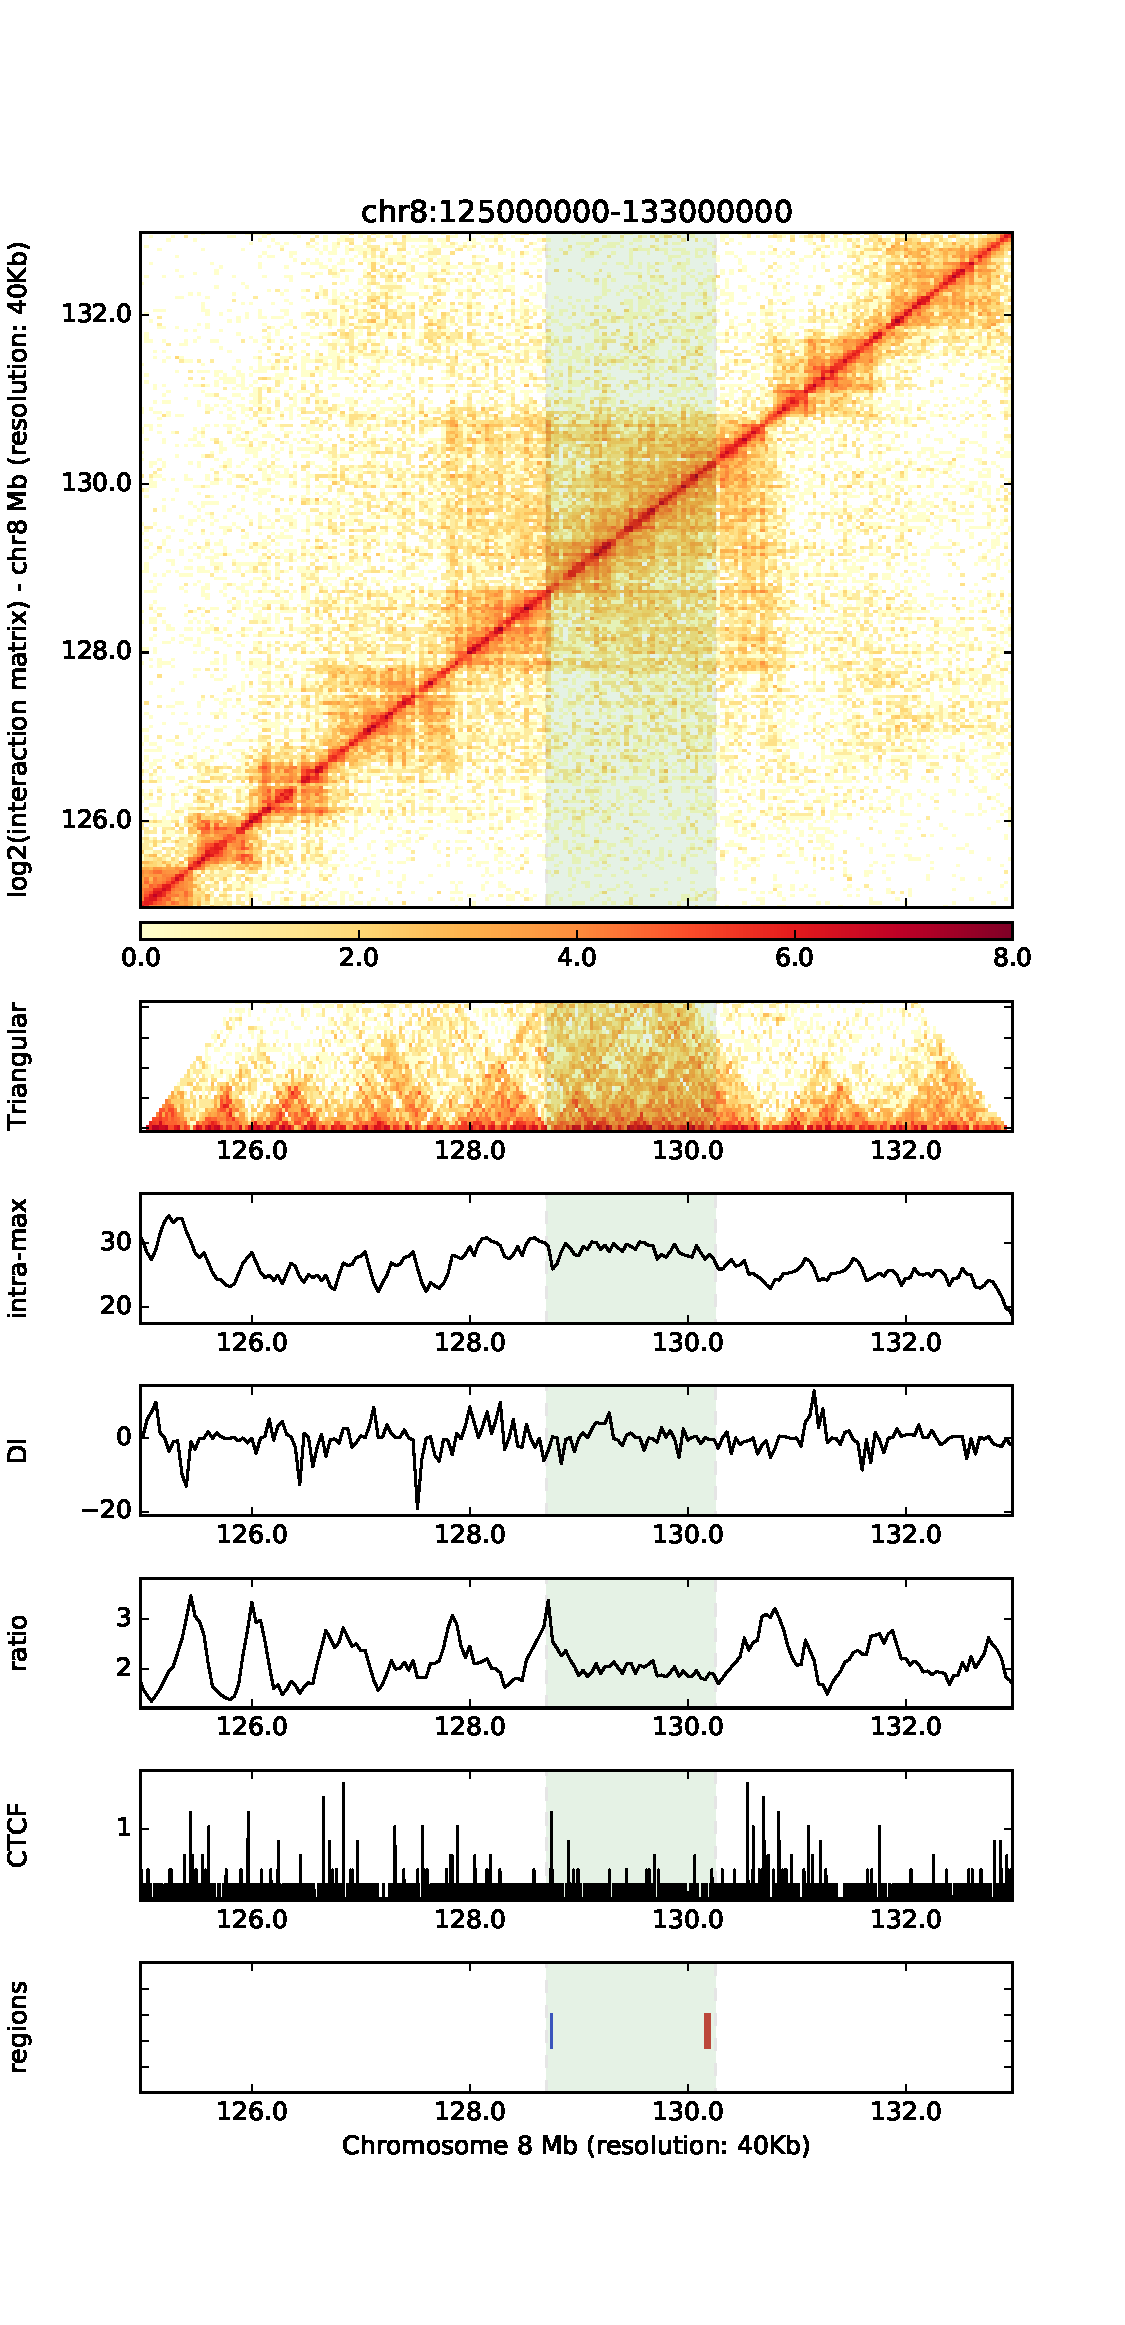
\includegraphics[width=\textwidth,height=\textheight,keepaspectratio]{figure/hicplotter_chr8-125000000-133000000}
    \caption{HiCPlotter sample output} %results/hicplotter.by_sample.standard/matrix-filtered.by_sample.res_40kb/filter.by_sample.standard/align.by_sample.bowtie2/CD34-HindIII-rep1/chr8\:125000000-133000000.pdf
    \label{fig:hicplotter_chr8}
\end{figure}
% \newpage
\clearpage